\vspace{12pt}
\section{Electrochemical Impedance Spectroscopy}

\subsection{Theory and overview}

Impedance spectroscopy is a powerful method for characterizing many of the conductive processes that take places within a material and between the material interfaces and electrodes. It is useful in the investigation of any kind of solid or liquid material and any kind of conduction process from electronic to ionic or mixed conduction as well as dielectric materials. A wide variety of materials such as electric or ionic ceramics, semiconductors, polymeric membranes, protective coatings, and thin films can be examined. Solid metal electrodes can be applied in many ways and the surrounding atmosphere is controlled to be either neutral, oxidizing or reducing, and humid or dry depending on the experiment. Impedance Spectroscopy is a useful technique for studying conduction in solids due to its ability under the right conditions to separate the various contributions to conductivity from within grains and across grain boundaries \cite{Barsoukov2005}. Impedance spectroscopy has been used in the study of solid ion conductors since Bauerle's first application of the technique on yttria stabilized zirconia (YSZ) \cite{Bauerle1969}.

 The basis of the method is to apply an electrical signal and measure the electrical response of the material over a range of frequencies. The overall electric response of the material results from the fundamental conduction processes, either electronic/ionic conduction or transfer between interfaces within the material. These fundamental processes are affected by the structural properties of the material, the composition in terms of grains or grain boundaries, the mobility of species within the different phases, and the availability of charge carriers and defects within the material. It is assumed that the properties affecting the conduction within the material and between the material and electrodes is time independent, and that all variables that affect conduction are controlled and form the basis of the particular study. Some parameters include temperature, surrounding gaseous atmosphere, applied bias voltage, or applied hydrostatic pressure.
 
 The electrical signal applied can take various forms such as an applied step voltage or random noise applied voltage, but these time variant techniques require Fourier transforming into the frequency domain in order to obtain an impedance. The more standard approach, and the one of this dissertation is to measure the impedance by applying a single frequency sinusoidal voltage signal and measuring the amplitude and phase shift of the current response using a Fourier transform of the response. This measurement can then be repeated over a range of frequencies available, typically in this study 1 Hz to 7 MHz. The material response is independent of applied bias voltage, and most experiments are conducted with a two symmetric electrodes. Thus the complex impedance can be measured from the known input signal having amplitude $V_0$ and angular frequency $\omega$, \[V = V_0\sin{\omega t}\] and the resulting current \[I(t) = I_0 \sin(\omega t + \phi).\] Then the impedance can be represented by a complex number as \[Z = Z' + i Z''\] with $Z'$ the real part and $Z''$ the imaginary part. These parts are related to the magnitude and phase by \[Z'=|Z|\cos{\phi} \hspace{1cm} Z''=|Z|\sin{\phi}.\] By plotting the imaginary part of impedance against the real part (the so-called ``Nyquist Plot''), the effectiveness of impedance spectroscopy can be easily seen in Figure \ref{meth:fig:eis:nyquist:ysz} as the results form a series of semicircular arcs along the real axis. Implicit in this method of plotting is that each data point is recorded at a different frequency and that frequency increases towards the origin moving along the real axis. 
\begin{figure}
    \centering
    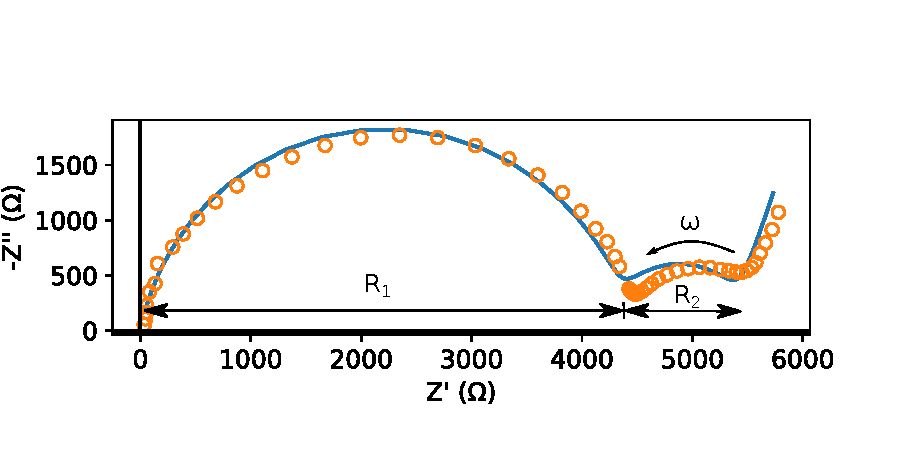
\includegraphics{Figures/190603-YSZ-nyquist-and-fit-edit.pdf}
    \caption{Nyquist plot of polycrystalline sample of yttria stabilized zirconia with equivalent circuit model fits.}
    \label{meth:fig:eis:nyquist:ysz}
\end{figure}
The distinctive arcs are formed as the result of different conduction mechanisms present in a polycrystalline material. Typically, the highest frequency arc is assigned to conduction within the grain of a material, while the middle frequency arc is assigned to conduction between adjacent grains or across grain boundaries. The lowest frequency arc is attributed to conduction process between the material and the electrodes. Each process can be modelled with an equivalent circuit, and those parameters, particularly resistance, can be used to determine the conductivity of the sample.

\vspace{12pt}
\subsection{Equivalent circuits and brick layer model}
The reasoning for this particular ordering can best be explained by the ``brick layer'' model of polycrystalline conduction. In the typical microstructure of a polycrystalline material, the grains of material are separated by small boundaries. In the brick layer model, these two phases along with the electrode connections are modeled with RC circuits in series with one another as seen in Figure \ref{fig:meth:RCRCmodel}. 
\begin{figure}
    \centering
    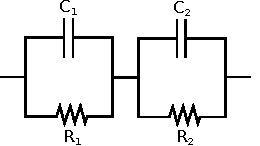
\includegraphics[width=.5\linewidth]{Figures/seriesLayerModel.pdf}
    \caption{Equivalent circuit for grain interior and grain boundary conduction process which yields characteristic two arc response in the Nyquist plot.}
    \label{fig:meth:RCRCmodel}
\end{figure}
The peaks of these arcs in the Nyquist plot are located at a characteristic frequency or time constant \begin{equation}
	\omega_0 = \frac{1}{RC} \hspace{.5cm} \mathrm{or} \hspace{.5cm} \tau_0 = RC
	\label{eq:meth:timeConstant}
\end{equation} which can also be seen as the maximum of the imaginary part of the impedance $Z''$ vs. frequency in Figure \ref{meth:fig:eis:bode:ysz}. In the brick layer model these characteristic frequencies are independent of the sizes of the grains or grain boundaries and are therefore constants of the conduction process and material itself (details of this are included in Appendix A). If two separate arcs can be resolved, the conclusion that the high frequency arc is the intra-grain conduction process is sound, while if only one arc is observed, no separation of the conduction process is possible, and only a total conduction can be determined.
\begin{figure}
    \centering
    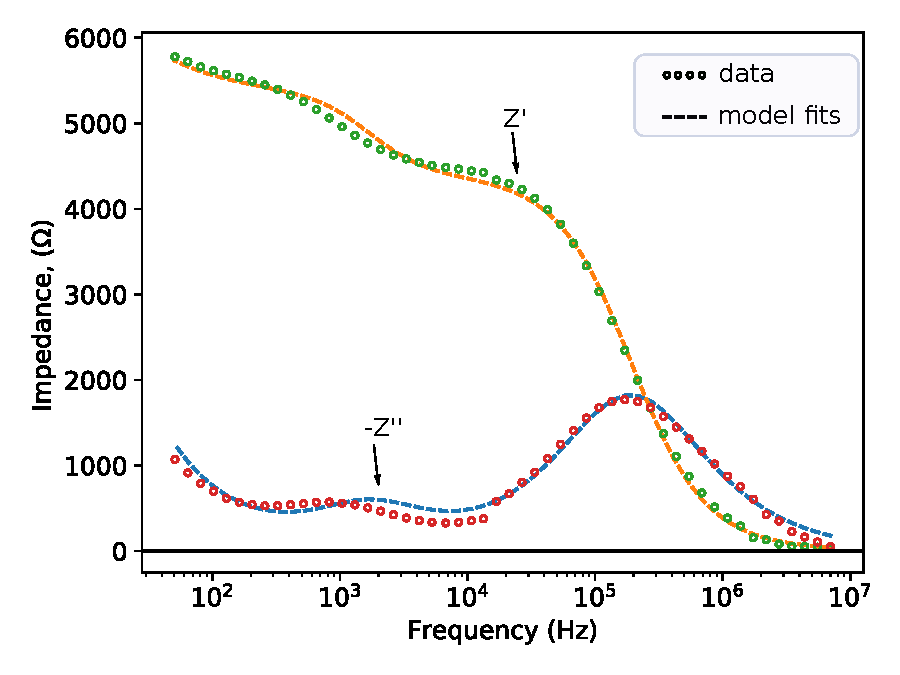
\includegraphics{Figures/190603-YSZ-bode-and-fit-edit.pdf}
    \caption{Real ($Z'$) and imaginary ($Z''$) parts of impedance of YSZ plotted against frequency. The peaks in the imaginary part correspond to the peaks in the semi-circular arcs in the Nyquist plot. Equivalent circuit model resulting from least squares fitting routine is also plotted.}
    \label{meth:fig:eis:bode:ysz}
\end{figure}
Equivalent circuits can be fit with least squares fitting routines. Numerous commercial software packages are readily available with built-in simple circuit fitting routines. We have utilized a custom routine for more complicated fits and higher data analysis throughput of fitting many data runs in succession. 

Impedance is modelled in the frequency domain using complex numbers according to the well known relationships:
\[\mathrm{Resistor: }Z_R(\omega)=R\]
\[\mathrm{Capacitor: }Z_C(\omega)=\frac{1}{i\omega C}\]
\[\mathrm{Inductor: } Z_L(\omega)=i\omega L\]
And combinations of these can be used with the usual rules of combining elements connected in series and in parallel.
\[Z_{\mathrm{E, series}} = Z_1+Z_2+...\]

\[\frac{1}{Z_{\mathrm{E, parallel}}} = \frac{1}{Z_1}+\frac{1}{Z_2}+...\]
The capacitance formula as stated is modified in practice to achieve a better fit. The arcs presented in the Nyquist plot are often depressed from an ideal semi-circular shape. By replacing the capacitor with a so called \emph{constant phase element} (CPE) a better fit is attained. The reason for this improvement is that when the constant phase element is paired with a parallel resistor, this models a case where a \emph{distribution} of time constants exist, due to inhomogeneities, variations in geometry and boundaries, and impurities. The impedance contribution from this element is \[Z_{\mathrm{CPE}}(\omega)=\frac{1}{Q(i\omega)^{n}}\] where $Q$ is a constant and the exponent $n$ is usually between 0.7 and 1 (1 represents an ideal capacitor) \cite{Orazem2002}. The true capacitance can then be found by \[C = R^{\frac{1}{n-1}}Q^{\frac{1}{n}}.\]

This evaluation of capacitance is important when it comes to carefully determining the conductivities that are attributed to intra-grain conductivity and across grain boundaries. For conductivity within the bulk of a grain the familiar equation 
\begin{equation}
    \sigma_{\mathrm{bulk}} = \frac{L}{A\cdot R_1}
\end{equation}
holds but for obtaining the grain boundary conductivity, as shown in Appendix A, under the brick layer model one must use
\begin{equation}
    \sigma_{\mathrm{GB}} =  \frac{C_1}{C_2}\frac{L}{A \cdot R_2}.
\end{equation}

\vspace{12pt}
\subsection{High Temperature Apparatus}

Our impedance spectrometer is a Bio-Logic SP-300 Potentiostat. Frequency ranges from 0.1 Hz to 7 MHz, and AC amplitudes from 20 mV to 1 V. Bias voltage from $-10$ to $+10$ V can be applied.   

The ability to perform impedance measurements at controlled high temperatures and environments is essential to the study of ionic conductivity. Figure \ref{fig:probostat} shows an apparatus for high temperature measurements that was developed as part of this research. The system consists essentially in a sample holder placed inside a split tube furnace. An alumina tube and stage apply pressure between platinum contacts and the sample using several stainless steel springs. The probe is inserted into a quartz tube that is sealed on each end with appropriate gas and vacuum fittings to maintain the desired atmosphere within the test chamber. Several geometries for sample placement were explored in our studies. Conductivity measurements were carried out in a controlled hydrogen-rich environment (5\% H$_2$ in N$_2$) as well as in ambient air, oxygen-rich and OH-saturated conditions. These various environments permit measurements of protonic, electronic, and mixed conductivity in our bulk and thin film samples. 

\begin{figure}
\centering
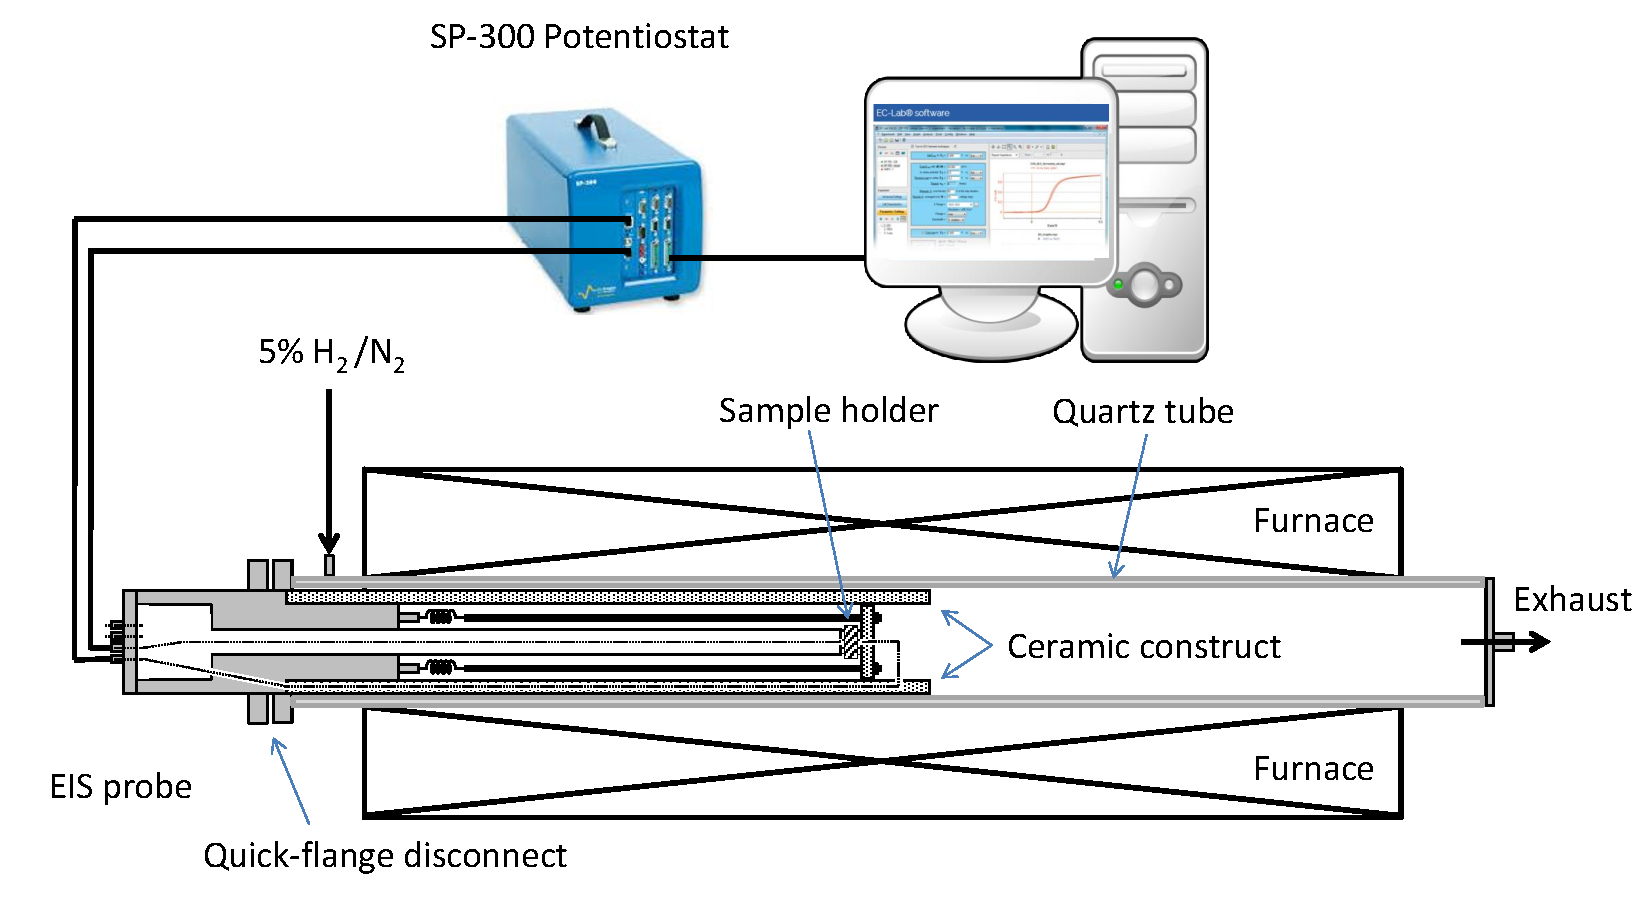
\includegraphics[width=\linewidth]{Figures/probostat.pdf}
\caption[High temperature electrical characterization apparatus]{Apparatus of high temperature conductivity measurements}
\label{fig:probostat}
\end{figure}

\vspace{12pt}
\subsection{Data fitting and parasitic inductance}
%Include data on YSZ as testing and verification of our setup.

One important factor to consider is the open cell behavior and the shorted behavior of the apparatus itself. We measure a significant inductive tail at very high frequencies that is inherent in the long wires and unshielded electromagnetic environment of the furnace. This inductive behavior can mask or distort the electrolyte resistance if the sample is itself of relatively low resistance. Measuring this parasitic inductance with a shorted configuration allows data taken on the electrolyte to be corrected. This correction has been shown to adjust resistance values by as much as 30\% \cite{Vladikova2006}. A simulated example of this can be seen in Figure \ref{meth:fig:inductanceCorrection}.

\begin{figure}[tb]
\centering
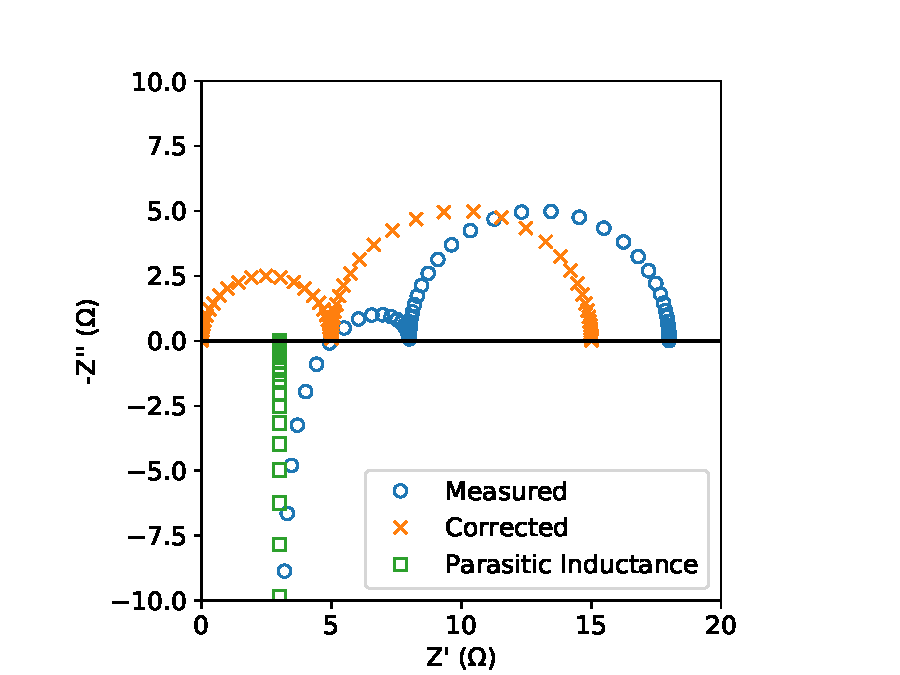
\includegraphics[width=.7\linewidth]{Figures/EIS-correction-sample.pdf}
\caption{Simulation of data correction for parasitic inductance}
\label{meth:fig:inductanceCorrection}
\end{figure}

\vspace{12pt}
\subsection{Sample preparation and contacts}
A very important aspect of taking these measurements is the application of high quality electrical contacts. Contacts need to adhere well throughout the contact area and also resist delamination from thermal stress during high temperature measurements. Ultimately contacts should be porous to allow gas phase element to be in close proximity to both the protonic conductor and electrical conductor. And the application of the contact must not compromise the integrity of the underlying oxide thin film. One of the most common and cost-effective techniques to apply porous contacts to oxide thin films is magnetron assisted D.C. sputtering. This technique was utilized in this  research. The basic elements and operation of a sputtering system assembled for this research is provided in Appendix B of this dissertation. 
